\chapter{Additional MNIST Results}
\label{app:mnist}

\paragraph{Learning Subsets.} We show the difference between seen and unseen data in more depth. Seen data are the feature points that were used by the neural network for training, unseen points were not used. Figure \ref{fig:mnist1000cnnsub} (a) shows that $\alpha$-linkage results in almost perfect clusterings for seen data for a large part of $\alpha \in [0,1]$. Also for using two (b), three (c) and five unseen characters (d), we achieve major improvements over using the raw pixel features.

\begin{figure}[h]
\centering
\begin{minipage}{.31\textwidth}
  \centering
  \subcaptionbox{The learned characters (i.e. labels $\{0,1,2,3,4\}$) can be clustered very well. Similar to training on all labels, the error goes down close to $0\%$.}
  {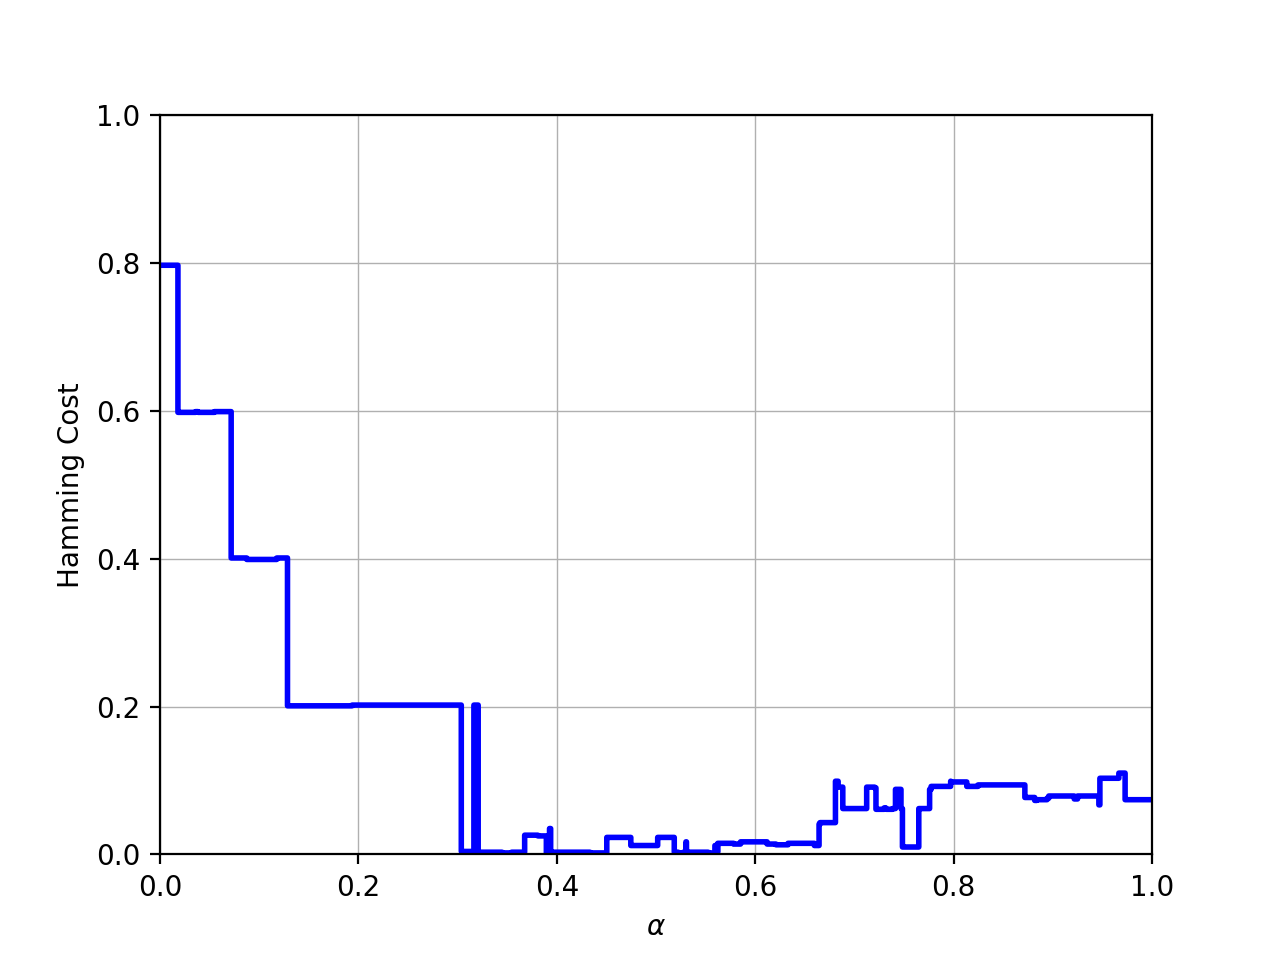
\includegraphics[width=\linewidth]{plots/mnist-cnn-sub-01234}}
\end{minipage}\quad
\begin{minipage}{.31\textwidth}
  \centering
  \subcaptionbox{Combining three trained ($0,2,4$) with two untrained digits ($6,8$) still leads to an optimal error of $2.1\%$ that is $10\%$ below complete linkage.}
  {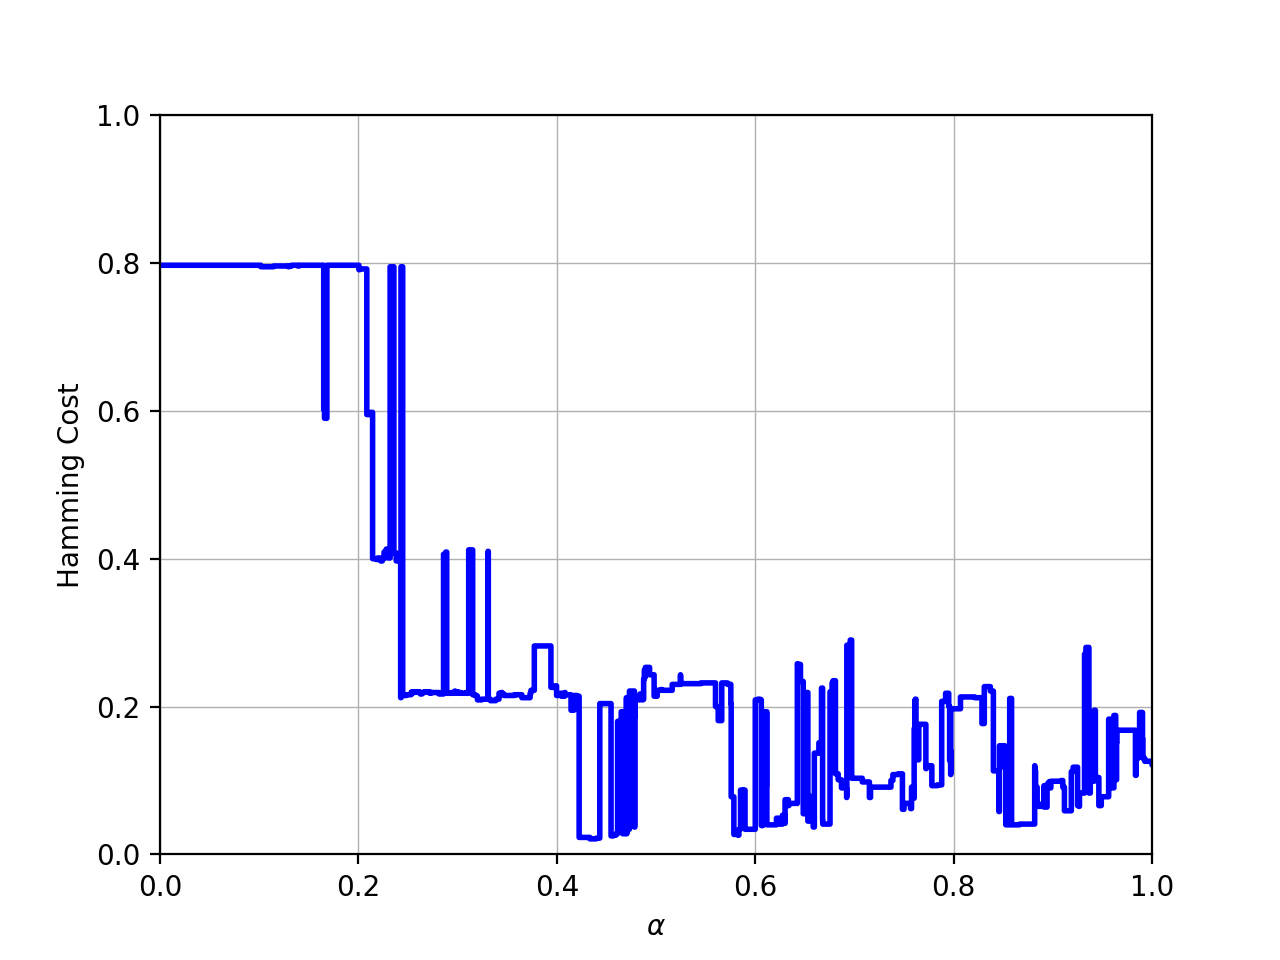
\includegraphics[width=\linewidth]{plots/mnist-cnn-sub-02468}}
\end{minipage}\quad
\begin{minipage}{.31\textwidth}
  \centering
  \subcaptionbox{Clustering three untrained ($5,7,9$) with two trained digits ($1,3$) already leads to larger errors of $15.1\%$, but still significantly less than for only unseen data.}
  {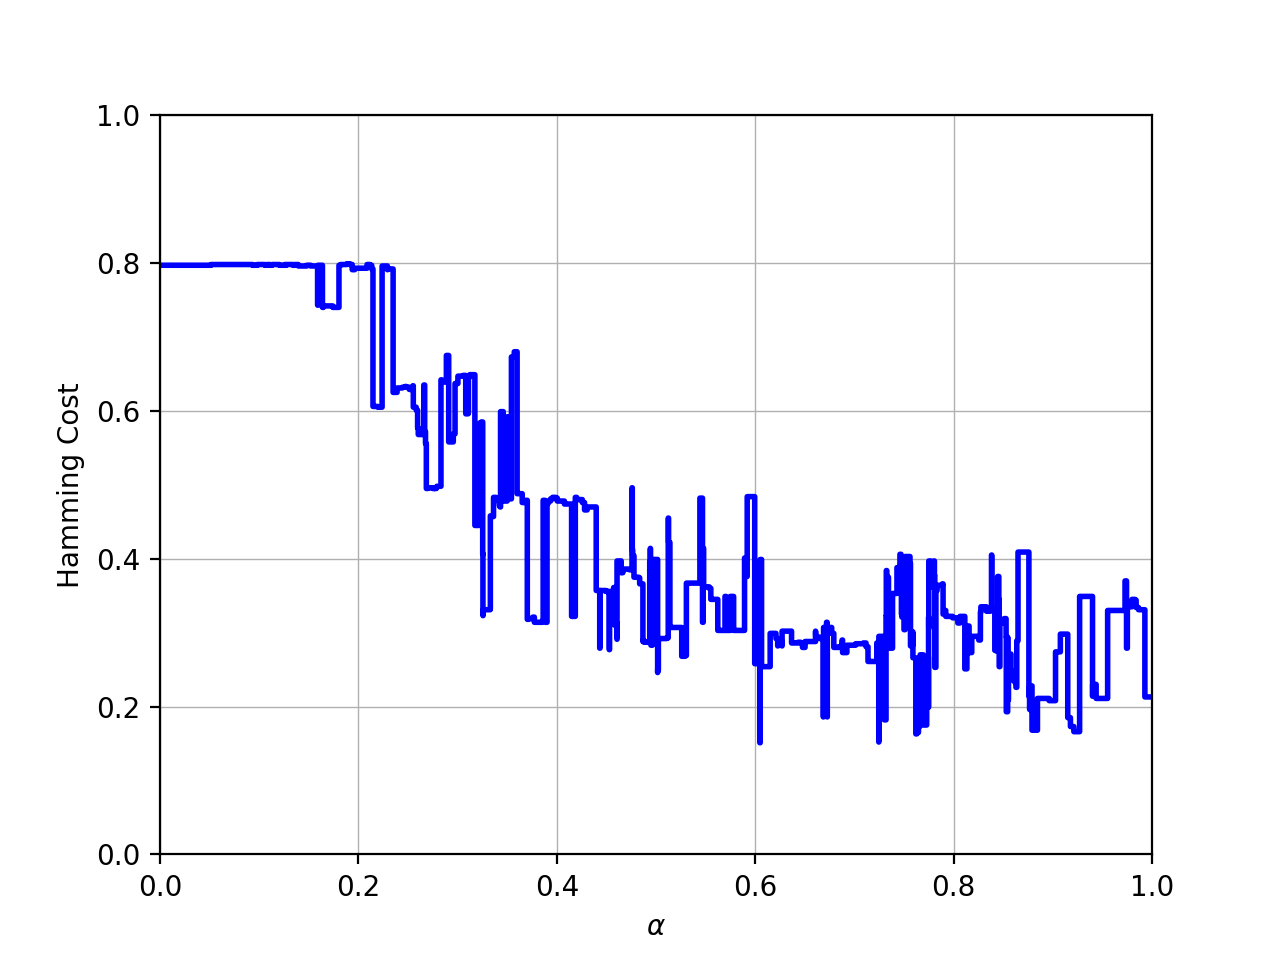
\includegraphics[width=\linewidth]{plots/mnist-cnn-sub-13579}}
\end{minipage}
\begin{minipage}{.31\textwidth}
  \centering
  \subcaptionbox{Even by clustering only untrained characters, the error goes down to $37\%$ that is a major improvement compared to clustering the raw pixel features that resulted in an optimal cost of $44\%$.}
  {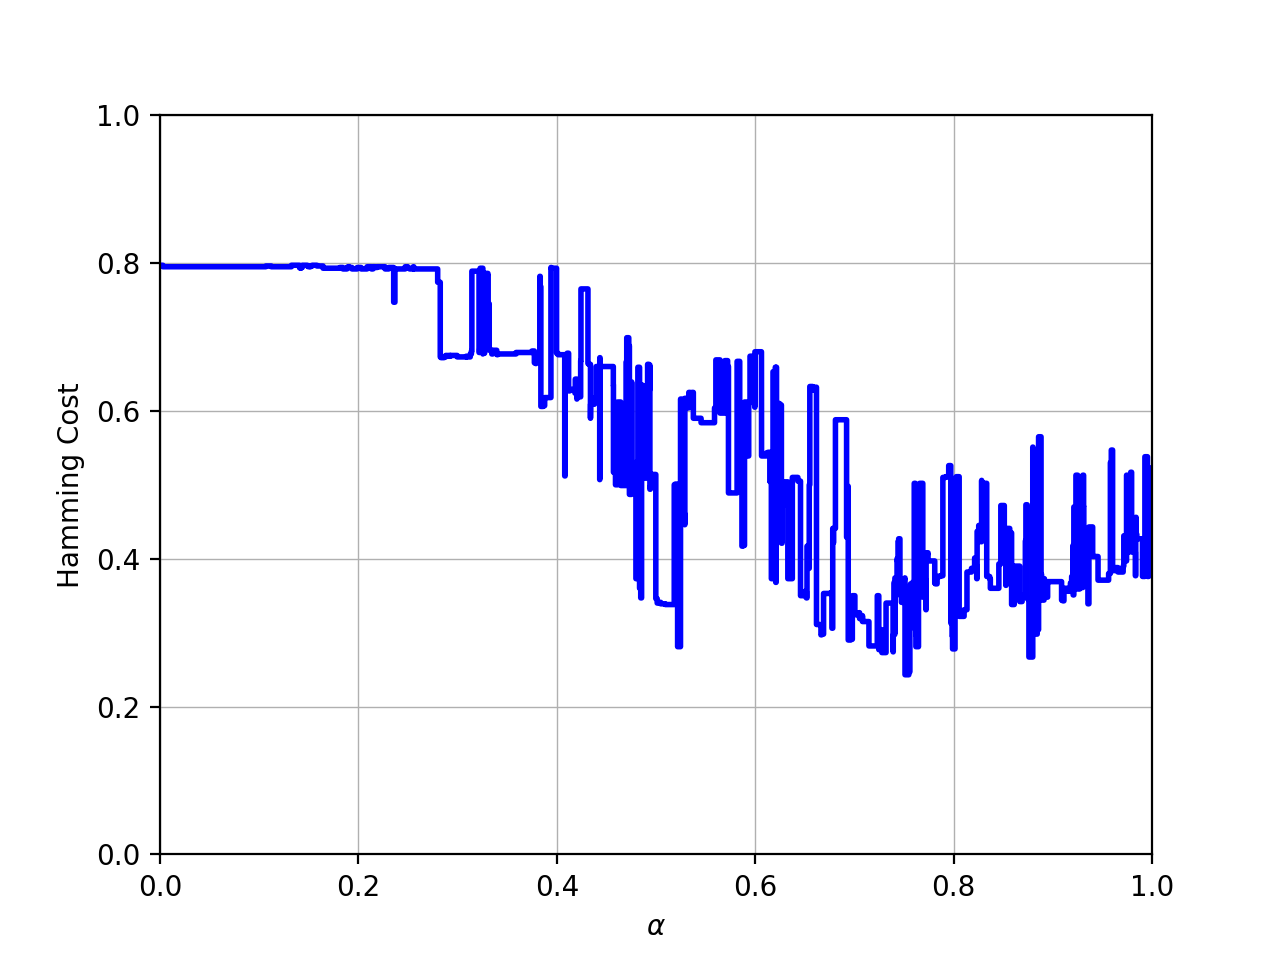
\includegraphics[width=\linewidth]{plots/mnist-cnn-sub-56789}}
\end{minipage}\quad
\begin{minipage}{.31\textwidth}
  \centering
  \subcaptionbox{Averaged over all 252 instances, the error for $\alpha_{opt} = 0.67$ is $20.7\%$ and an improvement of $1.4\%$ compared to complete linkage and $23\%$ compared to the raw pixel features.}
  {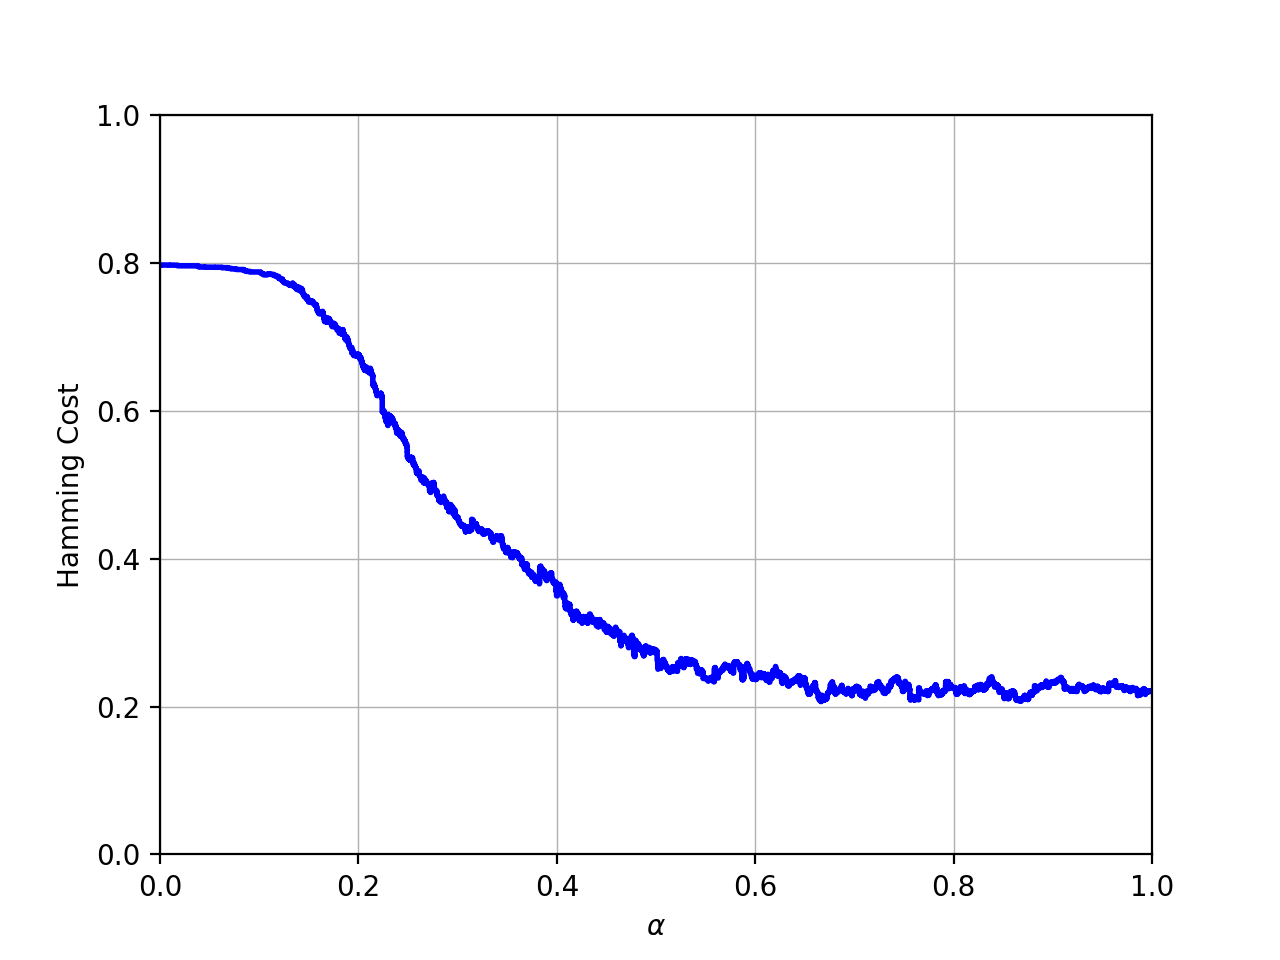
\includegraphics[width=\linewidth]{plots/mnist-cnn-sub-sc}}
\end{minipage}\quad
\begin{minipage}{.31\textwidth}
  \centering
  \subcaptionbox{Parameter advising results in major improvements for this setting. Using three values $\alpha^* \in \{0.86, 0.67, 0.99\}$ reduces the error by additional $5.3\%$ to $15.5\%$.} 
  {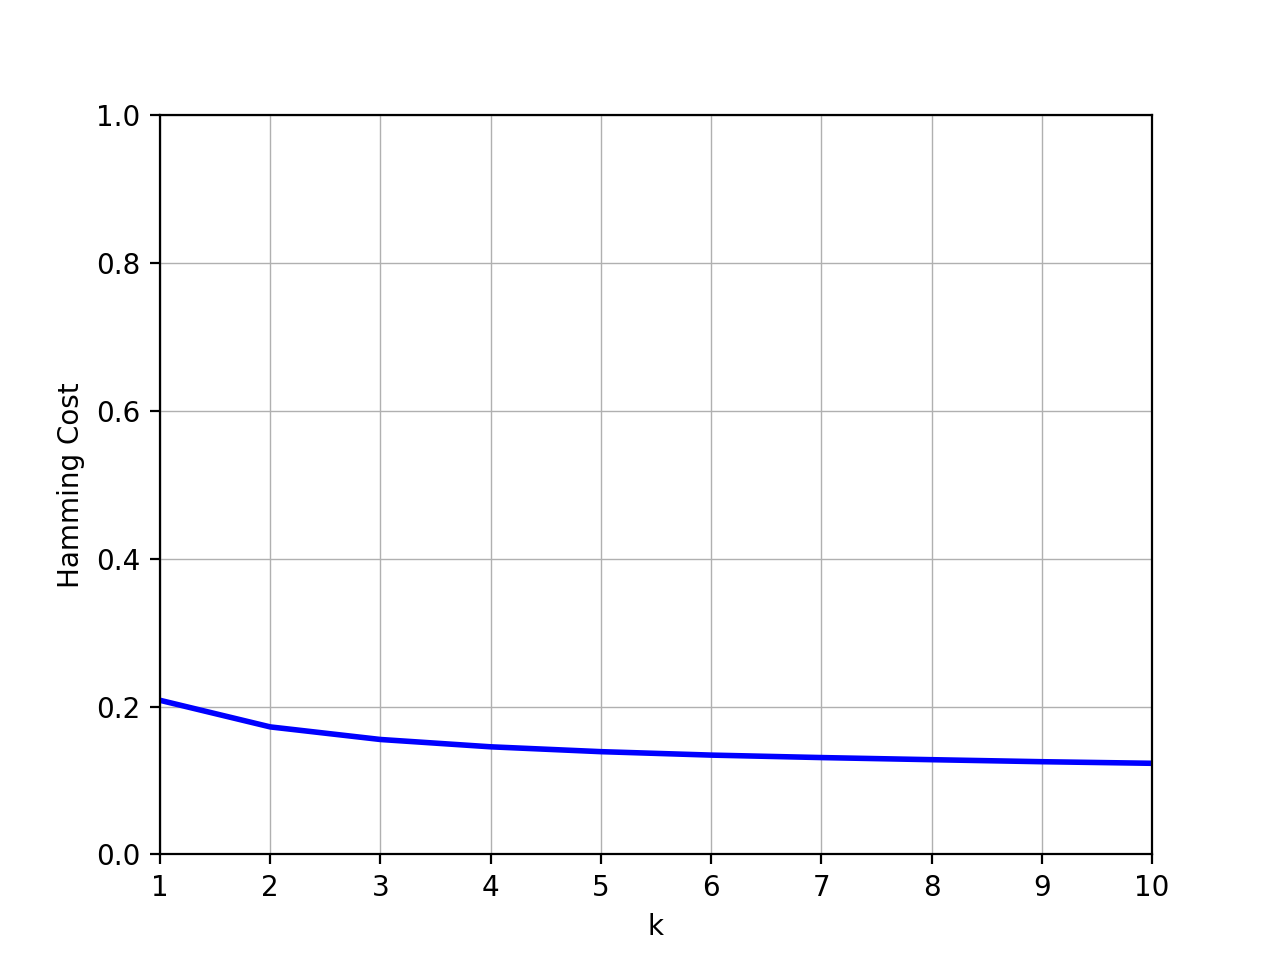
\includegraphics[width=\linewidth]{plots/mnist-cnn-sub-sc-top10}}
\end{minipage}
\caption{Learning features depending on a subset of the represented digits leads to different results for the MNIST data. While applying the learned digits still leads to almost perfect clusterings, clustering the unlearned digits leads to worse results that still are much better than using the raw pixel features.}
\label{fig:mnist1000cnnsub}
\end{figure}